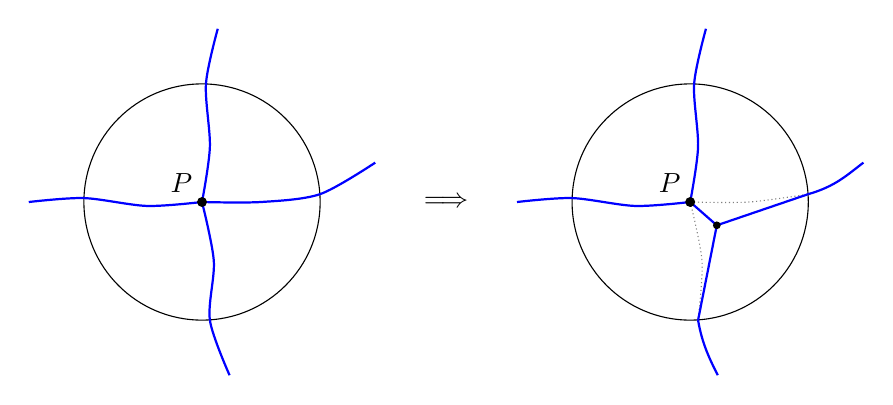
\begin{tikzpicture}[scale=1]
  % before: four arcs meet at P
  \begin{scope}
    \draw (0,0) circle (1.5);
    \draw[thick,blue] plot[smooth] coordinates {(0,0) (0.1,0.7) (0.05,1.5) (0.2,2.2)};
    \draw[thick,blue] plot[smooth] coordinates {(0,0) (-0.7,-0.05) (-1.5,0.05) (-2.2,0)};
    \draw[thick,blue] plot[smooth] coordinates {(0,0) (0.75,0.0) (1.5,0.1) (2.2,0.5)};
    \draw[thick,blue] plot[smooth] coordinates {(0,0) (0.15,-0.75) (0.1,-1.5) (0.35,-2.2)};
    \fill (0,0) circle (1.8pt) node[above left] {$P$};
  \end{scope}
  \node at (3.1,0) {$\Longrightarrow$};
  % after: P is split into two triple points
  \begin{scope}[xshift=6.2cm]
    \draw (0,0) circle (1.5);
    \draw[thick,blue] plot[smooth] coordinates {(0,0) (0.1,0.7) (0.05,1.5) (0.2,2.2)};
    \draw[thick,blue] plot[smooth] coordinates {(0,0) (-0.7,-0.05) (-1.5,0.05) (-2.2,0)};
    \draw[thick,blue] (1.5,0.1) .. controls (1.85,0.2) and (2.0,0.35) .. (2.2,0.5);
    \draw[thick,blue] (0.1,-1.5) .. controls (0.15,-1.8) and (0.25,-2.0) .. (0.35,-2.2);
    \draw[gray,densely dotted] plot[smooth] coordinates {(0,0) (0.75,0.0) (1.5,0.1)};
    \draw[gray,densely dotted] plot[smooth] coordinates {(0,0) (0.15,-0.75) (0.1,-1.5)};
    \draw[thick,blue] (0,0) -- (0.338,-0.296) -- (1.5,0.1);
    \draw[thick,blue] (0.338,-0.296) -- (0.1,-1.5);
    \fill (0,0) circle (1.8pt) node[above left] {$P$};
    \fill (0.338,-0.296) circle (1.4pt);
  \end{scope}
\end{tikzpicture}
